\documentclass[10pt,norsk,a4paper]{article}
\usepackage[utf8]{inputenc}
\usepackage[T1]{fontenc}
\usepackage[norsk]{babel}
% - PDF-relatert
\usepackage{hyperref,pdfpages,hypcap}
\hypersetup{colorlinks=true,allcolors=.}
\newcommand\fhref[2]{%
	\href{#1}{#2}\footnote{\url{#1}}%
}
% Andre pakker
\usepackage[cm]{fullpage}
\usepackage{parskip,multicol,textcomp,amssymb,graphicx,color,enumitem}
% - Korreksjon av fotnoter i seksjoner/overskrifter
\usepackage[stable]{footmisc}
% - Skrifttype
\usepackage[bitstream-charter]{mathdesign}
% - Kommentarer
\usepackage{comment}


\title{Generalforsamling \\
	Høsten 2018\\[3cm]
	
\includegraphics[width=0.5\textwidth]{cyb-logo.eps}\\[-.5cm]}
\date{14.\ november 2018}
\author{Cybernetisk Selskab}

% Blank header, samt footer med side x av y
\usepackage{fancyhdr}
\pagestyle{fancy}
\renewcommand{\headrulewidth}{0pt}
\fancyhead{}
\cfoot{Side~\thepage\ av~\pageref*{lastpage}}


\begin{document}

\maketitle{}
\newpage
\tableofcontents

\part*{Agenda}

\section{Valg av møteleder}

\section{Valg av referent}

\section{Valg av protokollunderskrivere}

\section{Valg av tellekorps}

\section{Godkjenning av innkalling}

\section{Godkjenning av dagsorden}

%\newpage

\section{Semesterberetninger}
\subsection{Semesterberetning ved leder}


\subsection{Semesterberetning ved kjellermogul}
\begin{multicols}{2}
Nå som semesteret snart er ferdig ser det ut til at høstsemesteret i 2018 har vært noen meget gode måneder for CYB og Escape.

Fadderuka, eller nytt av året - studiestartuka - var denne gangen veldig annerledes for CYBs del enn tidligere år.
Denne gangen tok vi på oss ekstra ansvar ved å ha skjenkebevilling samt utstyr fra Aass hos PSI.
Grunnen til at vi tok på oss dette var relatert til noen problemer med Placebos vanlige avtale med U1,
da U1 ikke får lov til å søke om bevilling hos Placebo samtidig som de utvider hos seg selv.
Fordi vi er i samme bydel var ikke dette problematisk for oss.
I forkant av studiestartuka ble det planlagt grundig hvordan dette skulle foregå.
Mandagen gikk supert, og vi hadde vår første dag med pub hos oss og Placebo.
Både Kafèdriften og pub i Escape gikk som vanlig.
Utrolig nok ble resultatet veldig bra hos Placebo, og generelt sett gikk alt der oppe i løpet av studiestartuka veldig bra!
Som vanlig var det problemer med kredittgrenser hos Vectura, men med mange ninja-bevegelser og en rask handling fra innkjøp og økonomi gikk dette egentlig veldig greit.
Omsetning både hos oss og Placebo gikk over all forventning.
Med det sagt så betyr det ikke at vi ikke har noen forbedringspunkter:
Vi kunne ha vært flinkere på føring av Z hos placebo, og vi kunne ha vært raskere med opprigg av ekstra bar i kantina både på gaffafesten og CTRL+ALT+DEL.
Avsluttende gikk P2P også helt supert for både oss og Placebo!

Resten av semesteret har vært preget av mange utlån og et generelt sett høyt aktivitetsnivå.
Escape har blitt benyttet til de vanlige arrangementene som brettspill, torsdagsklubb, fredagspub med mer.
De aller fleste arrangementene har gått meget bra, og mye av det kommer av at vi har hatt en "insider" i arrgruppa, nemlig arrkoordinator!
Dette har vist seg å være et praktisk verv for å proxye informasjon fra arr til resten av de relevante personene i KS.
Videre har vi fått en del folk fra RF som har vist interesse for enkelte av våre temafester (*kremt* HP-fest) og vi endte opp med noen av de bedre festene på lenge.
Tipp topp tommel opp til arr her!

Dagen@ifi ble flyttet en måned fram i tid dette semesteret sammenlignet med tidligere år.
Da undertegnede hadde avtalt et annet arrangement lenge før datoen for dette ble satt, så fikk vedkommende ikke mulighet til å være tilstede under dette.
Rapporter fra Dagen@ifi og KS har vært litt motstridene, men alt i alt virker det som om mesteparten egentlig gikk helt greit.
Igjen kunne vi ha vært mer effektive under oppsett av bar, så dette er noe jeg håper KS i framtiden kan se mer på.
Denne gangen ble det satt opp en midlertidig bar i biblioteket, som ble en helt OK løsning sammenlignet med 3. etg.
Dette er noe man burde ta med seg videre og utføre enda bedre i fremtiden!

SALUTT-kurset er et tema som har skapt mye usikkerhet den siste tiden for mer eller mindre alle kjellerpubene i Oslo.
Undertegnede var dum nok til å ta på seg rollen Gudfar i Cosa Nostra-sammarbeidet, og har derfor jobbet aktivt både på politisk og administrativt nivå.
Foreløpig jobbes det med å få i gang kursing i starten av januar,og med garantier fra næringsetaten om at dette ikke vil påvirke dagens bevilling.
Forhåpentligvis kaster mange funker seg på dette kurset.
Det jobbes aktivt med å sette opp en skreddersydd versjon av dette kurset,
og medlemmer av KS sitter i en arbeidsgruppe sammen med VT for å definere dette.
Det langsiktige målet her er å få et politisk unntak, som helt eller delvis unntar oss fra SALUTT-kravet.

Kjelleravtalen er også et tema som har dukket opp igjen.
Denne gangen har vi noe mer håndfast å ta tak i, så forhåpentligvis vil vi fra 1.1.19 ha en ny avtale.
Det jobbes for tiden aktivt med å avklare en del detaljer rundt denne.

Til slutt vil jeg takke for meg, og ikke minst takke for at KS har utført et veldig bra semester!
De interne som sørger for at driften går rundt fortjener også en god klapp på skuldern,
og alle i CYB har all grunn til å være stolte over det vi sammen har fått til.
For å hente opp det Karl skrev for 1 år siden:
\begin{blockquote}
Jeg er – som sikkert er sagt av mange før meg – veldig positiv til hva CYB kan få til framover og har fått til på ganske få år, og håper at vi en dag klarer å bli ikke bare en av de største, men den største kjellerforeningen ved Blindern.
\end{blockquote}
Det kan se ut til at dette er realiteten nå for tiden uten for mye spekulasjoner.
Så virkelig godt jobbet!
\end{multicols}

XOXO

\textbf{Adrian Helle}, \\
Kjellermogul \\
\date{14.\ november 2018}


%\newpage

\section{Kasserer orienterer}
\subsection{Regnskapets tilstand}
Kasserer presenterer regnskapet.

\subsection{Revidert budsjett for høsten 2018}
Kasserer presenterer budsjett.

\subsection{Foreløpig regnskap for våren 2018}
Kasserer presenterer foreløpig regnskap.

\subsection{Budsjett for 2019}
Kasserer presenterer budsjett.

\section{Kontigentfastsettelse}
Hovedstyret foreslår å holde medlemskontigenten på kr.~40,-.

\newpage

\section{Forslag til vedtektsendringer}

\subsection{Endring i forbindelse med antall }
\subsubsection{Forslag til endring av paragraf: §7h}
\begin{quote}
	\begin{enumerate}
		\item[§7h]
            ordinær generalforsamling avholdes i slutten av hvert semester.
            ekstraordinær generalforsamling avholdes når hovedstyret,
            \textcolor{red}{eller når minst 10 prosent eller 30 stykker av medlemmene ønsker det.}
	\end{enumerate}
\end{quote}

\subsection{Forslag om utestengelse}

\subsubsection{Forslag 1 ved Elise}
\subsubsubsection{Forslag til ny underparagraf: §2d}
\begin{quote}
    \begin{enumerate}
        \item[§2d] Hovedstyret jf. §5 kan ekskludere medlemmer som viser upassende oppførsel, som inkluderer, men er ikke begrenset til, seksuell trakassering, annen trakassering, mobbing eller utestengelse.
    \end{enumerate}
\end{quote}

\subsubsubsection{Forslag til ny underparagraf: §2e}
\begin{quote}
    \begin{enumerate}
        \item[§2e]
            Hovedstyret jf. §5 kan ekskludere eller etablere andre konsekvenser for medlemmer som bryter med medlemskriteriene jf. §2d.
            Konsekvensene burde samsvare med graden av overtredelse. Ved grov uaktsomhet kan medlemmer ekskluderes.
    \end{enumerate}
\end{quote}

\subsubsection{Forslag 2 ved Thor}
\subsubsubsection{Forslag til ny underparagraf: §2d}
\begin{quote}
    \begin{enumerate}
        \item[§2d]
            Medlemmer forventes å frastå fra upassende oppførsel, samt atferd som strider mot foreningens formål jf. §1.
            Upassende oppførsel inkluderer, men er ikke begrenset til, seksuell trakassering, annen trakassering, mobbing eller utestengelse.
    \end{enumerate}
\end{quote}

\subsubsubsection{Forslag til ny underparagraf: §2e}
\begin{quote}
    \begin{enumerate}
        \item[§2e]
            Hovedstyret jf. §5 kan ekskludere eller etablere andre konsekvenser for medlemmer som bryter med medlemskriteriene jf. §2d.
            Konsekvensene burde samsvare med graden av overtredelse. Ved grov uaktsomhet kan medlemmer ekskluderes.
    \end{enumerate}
\end{quote}

\subsubsection{Forslag 3 ved Andreas}
Jeg vil gjerne spille litt videre på Elise sitt forslag, og fremmer derfor et motforslag.

Samme budskap, men ønsker å ha en det formalisert om hvordan en eventuelt utestengelse skal foregå.
Jeg tenker at det er viktig at det ikke er lavere terskel for å kunne utestenge et medlem enn det er å stille mistillit til et styremedlem.
Utestengelse er et meget kraftig virkemiddel.

Sammen med disse nye vedtektene ønsker jeg også at HS skal utarbeide etiske retningslinjer før GF V19 som skal brukes grunnlag til utestengelse.

Frem til hovedstyret presenterer slike rettningslinjer foreslår jeg at en følger UiO sine etiske retningslinjer så langt som praktisk mulig for en studentforening.

\subsubsubsection{Forslag til ny paragraf: §11}
\begin{quote}
    \begin{enumerate}
        \item[§11a] Hovedstyret jf. §5 kan ekskludere medlemmer i kortere eller lenger periode hvis vedkommende har motarbeidet foreningens formål, eller nektet å innrette seg etter foreningens etiske retningslinjer.
        \item[§11b] Utestengelse vedtas av hovedstyret med 3/4 flertall.
        \item[§11c] Dokumentasjon av atferd hos medlem som vurderes utestengt skal rapporteres skriftlig til hovedstyret, i en slik form at det kan meddeles den som vurderes utestengt.
        \item[§11d] Spørsmålet om utestenging kan ikke avgjøres før medlemmet har blitt informert om omstendighetene som kan føre til utestenging, og blitt forelagt dokumentasjonen på den uakseptable atferden.
        \item[§11e] Beslutning om utestenging kan ikke tas før medlemmet har fått anledning til å ytre seg, innen en tidsramme som er avgjort av styret, minst 14 dager.
        \item[§11f] Ved utestengelse lenger enn 30 dager skal utestengelsen vedtas av generalforsamling etter lik prosedyre som §9.
        \item[§11g] Utestengelse med grunnlag i skjenkereglementet eller andre nærliggene grunner dekkes ikke av disse vedtekter og følger reglene til privat eiendomsrett.
    \end{enumerate}
\end{quote}

\newpage

\section{Valg}

\textit{
    Beklageligvis spesifiserte innkalling at arrangementssjef var oppe til valg.
    Dette stemmer ikke, og har blitt korrigert i dagsorden.
}

\begin{minipage}[t]{0.49\textwidth}
\subsection{Hovedstyret} %TODO Oppdater listen med verv
Man velges inn i hovedstyret for ett år av gangen.

\subsubsection{Kasserer}
\subsubsection{Kjellermogul}
\subsubsection{Promoteringssjef}
\subsubsection{Internansvarlig}
\subsubsection{Promoteringssjef}

\end{minipage}
\begin{minipage}[t]{0.49\textwidth}
\subsection{Kjellerstyret} %TODO Oppdater listen med verv
Alle verv som er til valg i kjellerstyret gjelder for ett semester av gangen. Med unntak av Økonomiansvarlig som blir valgt inn for to semester.

\subsubsection{Økonomiansvarlig}
\subsubsection{Innkjøpsansvarlig}
\subsubsection{Barsjef}
\subsubsection{Kafésjef}
\subsubsection{Teknisk ansvarlig}
\subsubsection{DJ-sjef}
\subsubsection{Utlånsansvarlig}
\subsubsection{Arrangementskoordinator}

\end{minipage}

\newpage

\section{Vedtektsendringer}
Forslag til vedtektsendringer legges ut nærmere generalforsamlingen.

\section{Æresmedlemskap}

\section{Utdeling av pins}

Arkivar deler ut pins.

\section{CYB50}

CYB har 50.~årsjubileum februar 2019, og ønsker i den sammenheng fortsatt frivillige til dette formålet. Leder for komitèen orienterer litt rundt planer sålangt.

Komitéen leter etter alle Ifi-studenter som ønsker å gjøre festuken i februar til en helspekket tidsperiode som kommer til å slukke alle faglige, interessante og sosiale tørster.

Interesse for deltagelse i arrangeringen kan sendes til \textbf{50@cyb.no}.


\part*{Vedlegg}\label{lastpage}
\addcontentsline{toc}{part}{Vedlegg}

\newpage
\phantomsection{}
\addcontentsline{toc}{section}{Vedtekter for Cybernetisk Selskab} % chktex
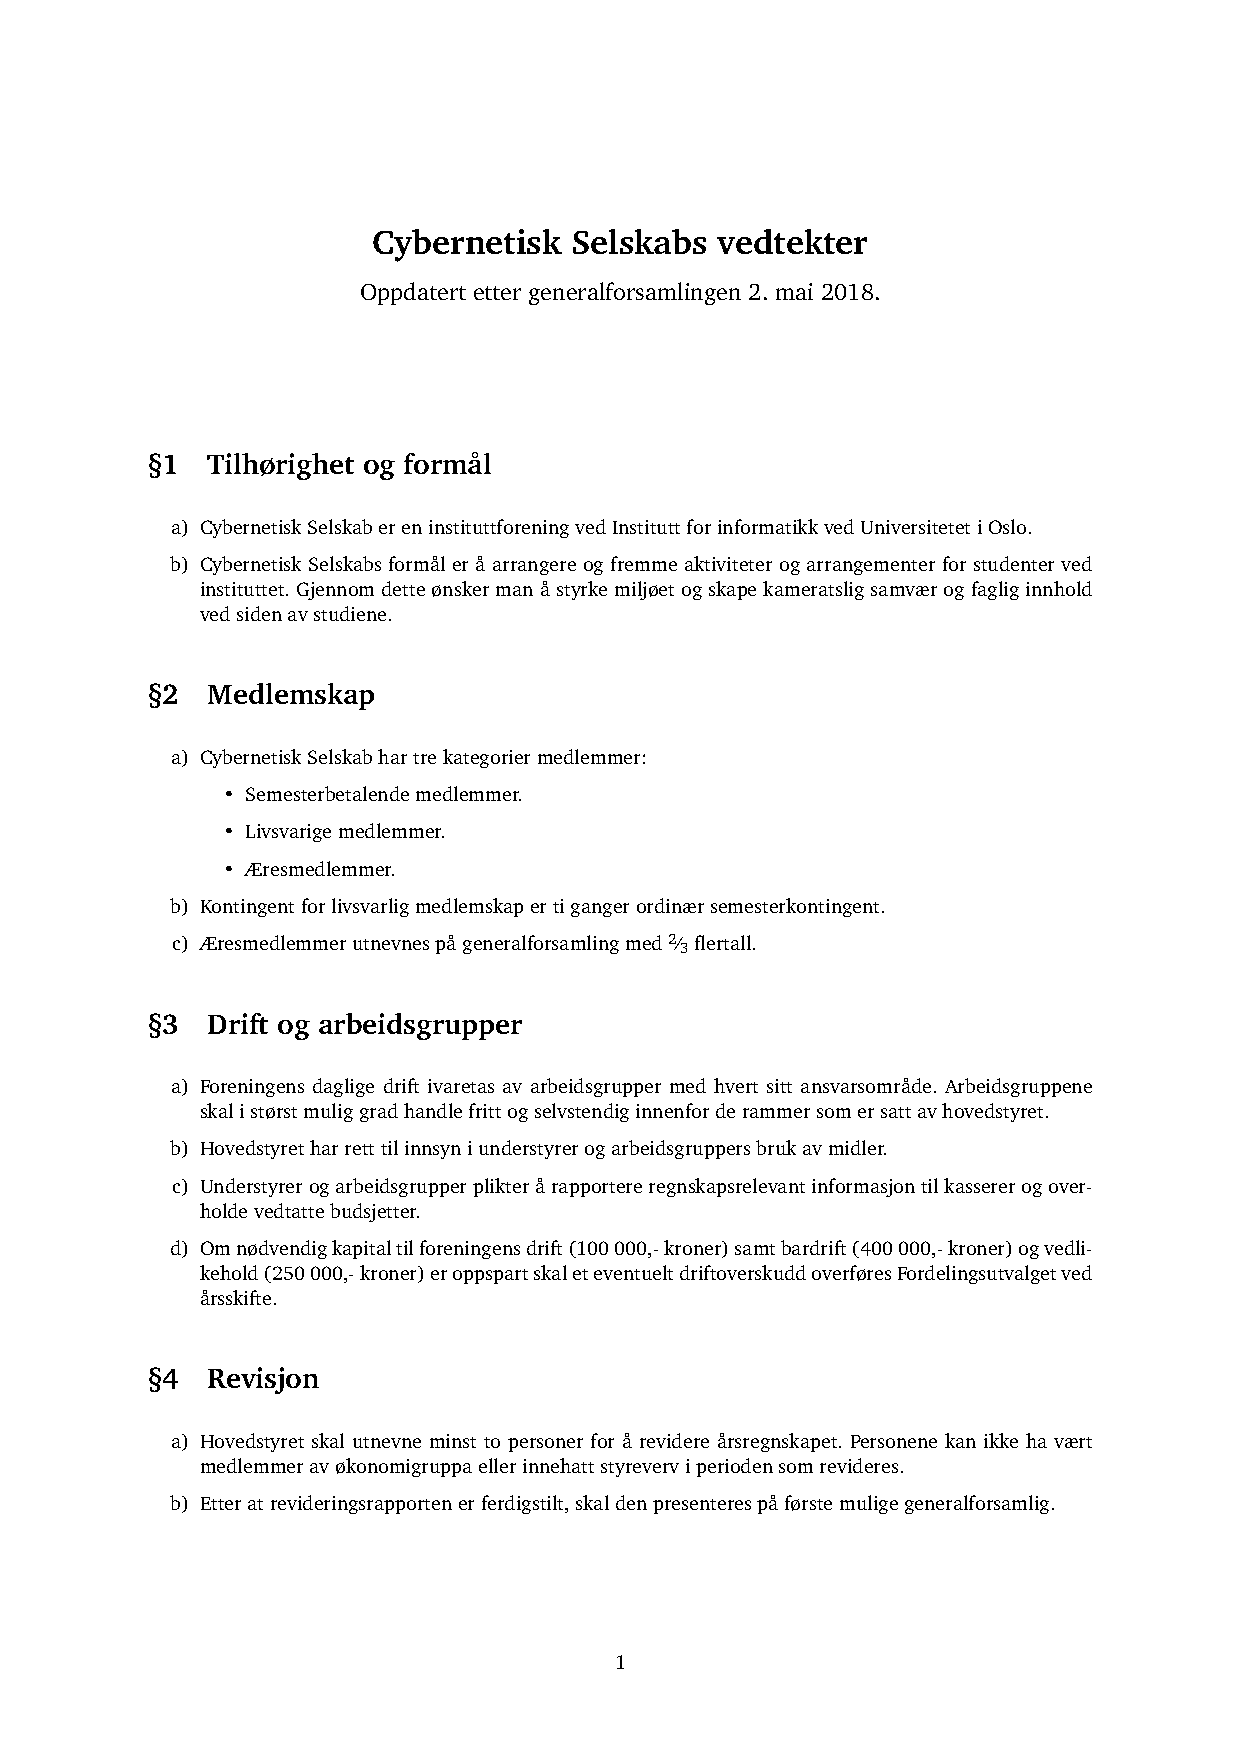
\includepdf[pages=-]{../vedtekter/vedtekter.pdf}

\end{document}
